% Created 2025-12-10 Wed 17:53
% Intended LaTeX compiler: pdflatex
\documentclass[a4paper, 11pt, colorlinks=true, citecolor=., linkcolor=black, urlcolor=black]{article}
\usepackage[utf8]{inputenc}
\usepackage[T1]{fontenc}
\usepackage{graphicx}
\usepackage{longtable}
\usepackage{wrapfig}
\usepackage{rotating}
\usepackage[normalem]{ulem}
\usepackage{amsmath}
\usepackage{amssymb}
\usepackage{capt-of}
\usepackage{hyperref}
\usepackage{fourier}
\usepackage{tikz}
\usepackage[ maxcitenames=1, maxbibnames=3,style=authoryear]{biblatex}
\addbibresource{references.bib}
\usepackage{subcaption}
\addbibresource{references.bib}
\author{Amitav Krishna}
\date{\today}
\title{Comparing Machine Learning Strategies for Quantum Noise Reduction}
\hypersetup{
 pdfauthor={Amitav Krishna},
 pdftitle={Comparing Machine Learning Strategies for Quantum Noise Reduction},
 pdfkeywords={},
 pdfsubject={},
 pdfcreator={},
 pdflang={English}}
\begin{document}

\maketitle
\emph{This is currently a work in progress. The todos will be removed once the training has been run.}
\section{Abstract}
\label{sec:orge2832a6}
Machine learning models for quantum state denoising must capture the nonlocal correlations inherent to density matrices. We compare convolutional and transformer autoencoders on synthetic density-matrix denoising across multiple noise channels. Noisy inputs have only 0.11 mean Uhlmann fidelity to their clean counterparts; the Frobenius-trained transformer recovers this to 0.95 (+0.84 improvement), while CNNs achieve only 0.30. Contrary to expectations, physics-informed regularization degrades reconstruction quality for both architectures—the physics-informed CNN performs worse than using the noisy input directly. These results establish architectural requirements for neural denoising of quantum states and caution against naive application of physics-based constraints.
\subsection{{\bfseries\sffamily DONE} Modify framing to an inversion of known noise channels}
\label{sec:orge9b636a}
\section{Introduction}
\label{sec:org9e417fc}
\subsection{{\bfseries\sffamily DONE} Add context on the state of ML-based noise reduction}
\label{sec:org0fce727}
Machine learning has rapidly become a major tool for mitigating quantum noise by learning direct mappings from corrupted measurement statistics or density matrices to cleaner quantum states. Early work used convolutional architectures to denoise mixed states by exploiting local spatial correlations in the density-matrix representation, demonstrating that even modest CNN autoencoders can partially reverse decoherence effects without any explicit knowledge of the underlying hardware noise channel\autocite{kendre2025machinelearningquantumnoise}. More recent approaches explore feedforward networks for reconstructing states corrupted by unknown dynamics, showing that neural approximators can serve as model-agnostic quantum noise suppressors \autocite{Morgillo_2024}. In parallel, several groups have focused on learning-based quantum state tomography, replacing traditional inversion with neural estimators that better tolerate measurement noise and incomplete data\autocite{PhysRevA.106.012409}.

Beyond tomography, machine learning has seen strong adoption in quantum error correction. Classical convolutional and multilayer perceptron decoders typically operate on local syndrome neighborhoods, which limits scalability and forces retraining when code distances change. Transformer-based QEC decoders were introduced to overcome this limitation, treating all stabilizer syndromes globally so that long-range correlations remain accessible to the model\autocite{wang2023transformerqecquantumerrorcorrection}. Related threads leverage reinforcement learning and optimal control networks to improve system robustness in closed-loop settings\autocite{Ma_2025}. Together, these developments reveal a field that has matured from proof-of-concept denoisers into a broad class of neural architectures that learn to suppress, correct, or compensate for noise across diverse quantum information tasks.
\subsection{{\bfseries\sffamily DONE} Add context on the current status quo for quantum error correction and quantum error mitigation.}
\label{sec:orgb4147ca}
Quantum computing research has coalesced around two complementary strategies for managing hardware noise. Quantum error correction provides a principled route to fault-tolerant computation by encoding logical information into larger composite systems and continuously detecting and correcting physical errors \autocites{202509.2149}[][]{Bravyi_2024}. In theory, this approach supports arbitrarily long computations with bounded overhead once physical error rates fall below a threshold \autocites{2024}[][]{202509.2149}. However, present devices remain significantly above those thresholds, and the resource costs associated with real-time decoding and large code distances limit practical deployment \autocites{Bravyi_2024}[][]{202509.2149}.

Quantum error mitigation offers an alternative aligned with current hardware constraints. It reduces the impact of noise through circuit-level extrapolation, classical inference, and statistical post-processing, allowing experiments to extract more reliable observables without modifying the underlying qubit architecture \autocites{Bultrini_2023}[][]{RevModPhys.95.045005}. Unlike QEC, mitigation does not guarantee correctness at scale, and its cost typically grows rapidly with circuit depth and system size \autocites{RevModPhys.95.045005}[][]{filippov2024scalabilityquantumerrormitigation}. As a result, QEM serves as the standard tool for near-term applications, while progress in QEC continues to define the long-term path toward fully fault-tolerant quantum computation\autocites{Bultrini_2023}[][]{202509.2149}.
\section{Related implementations}
\label{sec:orgf83def0}
Recent work has explored convolutional autoencoders for density-matrix denoising. Kendre et al. introduced a CNN-based approach that treats the density matrix as a two-channel image and applies standard encoder-decoder convolutions to map noisy states to clean reconstructions \autocite{kendre2025machinelearningquantumnoise}. This architecture exploits local spatial correlations but cannot directly model the nonlocal quantum correlations present in entangled states. Morgillo et al. used feedforward networks for states corrupted by unknown noise channels, demonstrating model-agnostic denoising but without addressing architectural limitations \autocite{Morgillo_2024}. However, neither approach has been systematically compared to architectures capable of modeling nonlocal correlations.

An alternative thread enforces physical validity through hard constraints. Hradil et al. proposed positivity-constrained feedforward networks that project outputs onto the space of valid quantum states, guaranteeing Hermiticity and positive semidefiniteness by construction \autocite{PhysRevA.106.012409}. While this ensures physical consistency, it does not address whether the network itself learns representations suited to quantum structure.

Transformer architectures have been explored for related quantum tasks but not for density-matrix denoising. Wang et al. introduced Transformer-QEC for syndrome decoding in quantum error correction, demonstrating that self-attention enables global receptive fields that outperform local CNN decoders \autocite{wang2023transformerqecquantumerrorcorrection}. Their work motivates our hypothesis that attention mechanisms may similarly benefit density-matrix reconstruction, where nonlocal correlations are fundamental.

No prior work has directly compared convolutional and attention-based architectures for density-matrix denoising under controlled conditions, nor evaluated the impact of physics-informed regularization on reconstruction quality. Our experiments address both gaps.
\section{Methods}
\label{sec:orgd203aab}
\subsection{Dataset}
\label{sec:orga8fc240}
All experiments use 5-qubit quantum states, each represented as a 32 \(\times\) 32 density matrix since the Hilbert space of an \emph{n}-qubit system has dimension \(2^n\). Clean states are generated by sampling random quantum circuits with depths uniformly drawn from 6 to 9 layers. Each layer applies (i) a single-qubit gate chosen uniformly from \(\{X, Y, Z, H, T, S, R_x(\theta), R_y(\theta), R_z(\theta)\}\) with \(\theta \sim \mathcal{U}(0, 2\pi)\), followed by (ii) two randomly selected adjacent two-qubit gates from \(\{CNOT, CZ, SWAP\}\). This produces moderately deep circuits with nontrivial entanglement structure.

Noise is injected by applying a stochastic noise channel after every moment of the circuit. We evaluate five noise types: depolarizing, amplitude damping, phase damping, bit-flip, and a mixed channel. Each noise channel is implemented as a Cirq\autocite{CirqDevelopers_2025} noise operation applied independently to every qubit at each moment, with strength \emph{p} \(\in {0.05, 0.10, 0.15, 0.20}\). All simulations use Cirq's double-precision (\texttt{dtype=np.complex128}). The mixed noise channel is a sequential composition of depolarizing, amplitude-damping, phase-damping, and bit-flip channels, each applied with strength \emph{p} /4. Clean states \(\rho_{clean}\) are obtained by simulating the noiseless circuit using Cirq's \texttt{DensityMatrixSimulator}, and noisy states \(\rho_{noisy}\) are obtained by re-simulating the same circuit with noise inserted at every moment.

The dataset was originally generated with one million ($\backslash$(\(\rho\)\textsubscript{clean},\(\rho\)\textsubscript{noisy}) pairs (50,000 samples for each of the 20 noise-type / noise-level combinations). For computational efficiency, we use a uniformly subsampled subset of 100,000 examples in all experiments. The subsampling is stratified across noise types and noise levels, preserving the exact per-cell distribution of the original dataset. As a result, the statistical properties of the training data are unchanged, and all reported results reflect the same underlying data distribution as the original dataset. As a result, the statistical properties of the training data are unchanged and all reported results reflect the same underlying data distribution as the full one-million-sample dataset. Each density matrix is stored in a two-channel real/imaginary representation suitable for neural-network processing.

The noise channels follow their standard Kraus-operator definitions\autocite{nielsen_chuang_2010}. For depolarizing noise,

$$
\mathcal{E}_{dep}(\rho) = (1-p)\rho + \frac{p}{3}(X \rho X + Y \rho Y + Z \rho Z)
$$
Amplitude damping uses

$$
K_0 = \begin{pmatrix}
1 & 0\\
0 & \sqrt{1-p}
\end{pmatrix}, 
 K_1 = \begin{pmatrix}
0 & \sqrt{p}\\
0 & 0
\end{pmatrix}
$$
Phase damping applies

$$
K_0 = \sqrt{1-p}I, & K_1 = \sqrt{p}Z.
$$
Bit flip noise is

$$
\mathcal{E}_{bf}(\rho) = (1-p)\rho + p X \rho X.
$$

As previously stated, the mixed channel applies these four channels sequentially, each with strength \emph{p} /4.
\subsection{Convolutional Autoencoder}
\label{sec:org5816bb5}
The convolutional autoencoder is inspired by the architecture introduced in \autocite{kendre2025machinelearningquantumnoise} for density-matrix denoising. The model treats each 32×32 complex-valued density matrix as a two-channel image (real and imaginary components), enabling the network to exploit the local spatial patterns created by different quantum noise channels. The encoder consists of a sequence of convolutional blocks with ReLU activations and 2×2 max-pooling, progressively reducing spatial resolution while expanding the channel dimension (2→48→96→192). The decoder mirrors the encoder through nearest-neighbor upsampling and transposed convolutions, reconstructing the full resolution density matrix. A final convolutional layer projects the output back to two channels representing the real and imaginary components.
\subsection{Transformer Autoencoder}
\label{sec:orga9cac67}
The Transformer autoencoder models each 32×32 complex-valued density matrix as a sequence of token embeddings, where each token corresponds to one element in the row-vectorized matrix, with real and imaginary parts. This architecture allows every element in the input to attend globally to every other element, preserving the \emph{non-local} structure characteristic of entangled quantum states. The encoder consists of a stack of Transformer encoder layers with multi-head self-attention, enabling the model to capture global correlations across the entire state. The encoded sequence is compressed through a symmetric bottleneck module that projects the embedding dimension down and back up, serving as a latent representation. The decoder comprises Transformer decoder layers that apply both self-attention within the output sequence and cross-attention to the encoder memory. A linear projection generates the reconstructed sequence, which is reshaped into a 2D matrix.
\subsection{Normalized Frobenius fidelity loss}
\label{sec:org795736f}
The reconstruction loss used in our experiments is a normalized Frobenius inner product that measures the correlation between predicted and target density matrices. For each predicted–target pair of density matrices (\(\hat{\rho}\)) and (\(\rho\)), the loss is computed as
$$
\mathcal{L}_{\text{fid}}(\hat{\rho}, \rho) = 1 - \frac{\mathrm{Re}\langle \hat{\rho}, \rho \rangle_F}{\lVert \hat{\rho} \rVert_F \cdot \lVert \rho \rVert_F}
$$
where (\(\langle \hat{\rho}, \rho \rangle_F = \mathrm{Tr}(\hat{\rho}^\dagger \rho)\)) is the Frobenius inner product and (\(\lVert \cdot \rVert_F\)) is the Frobenius norm. This formulation is analogous to cosine similarity for complex matrices: it measures the alignment between predicted and target states while normalizing for magnitude differences. The loss is bounded between 0 and 2, achieving 0 when the matrices are perfectly aligned and 2 when they are maximally anti-correlated.

Unlike the squared Frobenius distance (\(\lVert \hat{\rho} - \rho \rVert_F^2\)), the normalized fidelity is scale-invariant and focuses on structural similarity rather than absolute elementwise error. This property is desirable for density-matrix reconstruction, where preserving the relative structure of coherences matters more than matching raw magnitudes. The Uhlmann fidelity remains the correct operational measure of quantum state distinguishability, but its reliance on matrix square roots and diagonalization makes it orders of magnitude more expensive to evaluate during training. The normalized Frobenius fidelity provides a computationally efficient proxy that correlates well with reconstruction quality while remaining compatible with gradient-based optimization.
\subsection{Physics-informed loss}
\label{sec:orgc02bd21}

The physics term enforces the basic structural axioms of a valid density matrix during reconstruction. Given a predicted state (\(\hat{\rho}\)), the loss penalizes violations of Hermiticity, trace normalization, and positive semidefiniteness, which are the three core constraints defining legitimate quantum states. Hermiticity is enforced by measuring the deviation between (\(\hat{\rho}\)) and its conjugate transpose, trace preservation is encouraged by penalizing deviations of (\(\mathrm{Tr}(\hat{\rho})\)) from unity, and positivity is promoted by penalizing negative eigenvalues of (\(\hat{\rho}\)). Together, these terms guide the model toward producing physically consistent outputs, irrespective of the noise model or architecture.

Formally, 
$$
\mathcal{L}_{physics}(\hat{\rho})
= \lambda_{\mathrm{herm}} \left|\hat{\rho} - \hat{\rho}^\dagger\right|_2^2 +
\lambda_{\mathrm{trace}},\big(\mathrm{Tr}(\hat{\rho}) - 1\big)^2 +
\lambda_{\mathrm{psd}},\big| \min(0,, \lambda_i(\hat{\rho})) \big|_2^2 ,
$$

where (\(\lambda_i(\hat{\rho})\)) are the eigenvalues of (\(\hat{\rho}\)). The total training loss combines this term with the normalized fidelity loss

$$
\mathcal{L}_{total} = \mathcal{L}_{\text{fid}}(\hat{\rho}, \rho) + 0.1 \cdot \mathcal{L}_{physics}(\hat{\rho}).
$$

The physics term is weighted by 0.1 to prevent it from dominating the reconstruction objective during early training.
\subsubsection{{\bfseries\sffamily TODO} Citation needed on that loss}
\label{sec:org7ee6a3a}
\section{Experimental Design}
\label{sec:orgf76e7b7}
We evaluate the four denoising configurations under a controlled and reproducible simulation pipeline designed to isolate the effects of architecture and loss function. All models are trained to map noisy density matrices to their clean counterparts using identical optimization settings. Training uses the Adam optimizer with a learning rate of 3e-4, a batch size of 8 for the transformer and 32 for the CNN, and a fixed budget of 100 epochs. Weight initialization follows PyTorch defaults, and a validation split of ten percent of the training set is used for checkpoint selection based on validation loss. Each model is trained using PyTorch's default random initialization.

Evaluation is performed on the held out test set using multiple metrics. These include Uhlmann fidelity between the reconstructed and target states, Frobenius reconstruction error, trace deviation, Hermiticity deviation, and the magnitude of any negative eigenvalues. This combination of metrics allows us to assess both denoising performance and physical validity. Model capacities are kept comparable across architectures by matching parameter counts within ten percent.
\subsection{Hyperparameters}
\label{sec:orgad67cee}

\subsubsection{Shared Hyperparameters}
\label{sec:orga98b653}

\begin{center}
\begin{tabular}{ll}
Component & Value\\
\hline
Optimizer & Adam\\
Learning rate & 3e-4\\
Weight decay & 0\\
Epochs & 100\\
Checkpoint selection & Best validation loss\\
Dataset size & 100,000 circuits\\
Train/validation/test split & 80/10/10\\
\end{tabular}
\end{center}
\subsubsection{Architecture-Specific Hyperparameters}
\label{sec:org35ecf9c}
\begin{center}
\begin{tabular}{lll}
Component & Convolutional Autoencoder & Transformer Autoencoder\\
\hline
Input representation & 32 \(\times\) 32 \(\times\) 2 & 1024 tokens (real/imag)\\
Embedding / channels & 2 \(\rightarrow\) 48 \(\rightarrow\) 96 \(\rightarrow\) 192 & Linear 2 \(\rightarrow\) 32\\
Batch size & 32 & 8\\
Encoder depth & 3 conv blocks & 4 layers, 4 heads\\
Decoder depth & 3 conv blocks & 4 layers\\
Kernel size & 3 \(\times\) 3 & -\\
Pooling & MaxPool 2 \(\times\) 2 & -\\
Upsampling & Nearest neighbor & -\\
MLP hidden size & — & 64\\
Dropout & — & 0.1\\
Bottleneck & — & Linear 32 \(\rightarrow\) 16 \(\rightarrow\) 32\\
Output projection & ConvTranspose2d(48 \(\rightarrow\) 2) & Linear 32 \(\rightarrow\) 2\\
Activation & ReLU & GELU\\
Parameter Budget & \textasciitilde{}500k & \textasciitilde{}500k\\
\end{tabular}
\end{center}
\emph{We avoid patch embeddings in the Transformer to preserve element-level nonlocal structure; patching would impose a locality bias that conflicts with the architectural comparison.}
\subsection{{\bfseries\sffamily TODO} Add details on compute used}
\label{sec:org3183dca}
\subsubsection{It was an RTX A4000}
\label{sec:org6c29113}
\newpage
\section{Results}
\label{sec:orga8ac61e}
Transformers outperform CNNs by one to two orders of magnitude in fidelity, while physics-informed losses stabilize weaker models and constrain stronger ones. Across noise types and noise levels, transformer models retain structure that CNNs consistently lose, and the physics-informed variant trades peak performance for robustness under heavy corruption. These patterns appear consistently across training curves, test metrics, and noise-resolved evaluations, and they frame the detailed comparisons presented in the sections that follow.
\subsubsection{Training Dynamics and Convergence Behavior}
\label{sec:org7f4fcad}
\begin{figure}[h!]
\centering
\begin{subfigure}{0.45\linewidth}
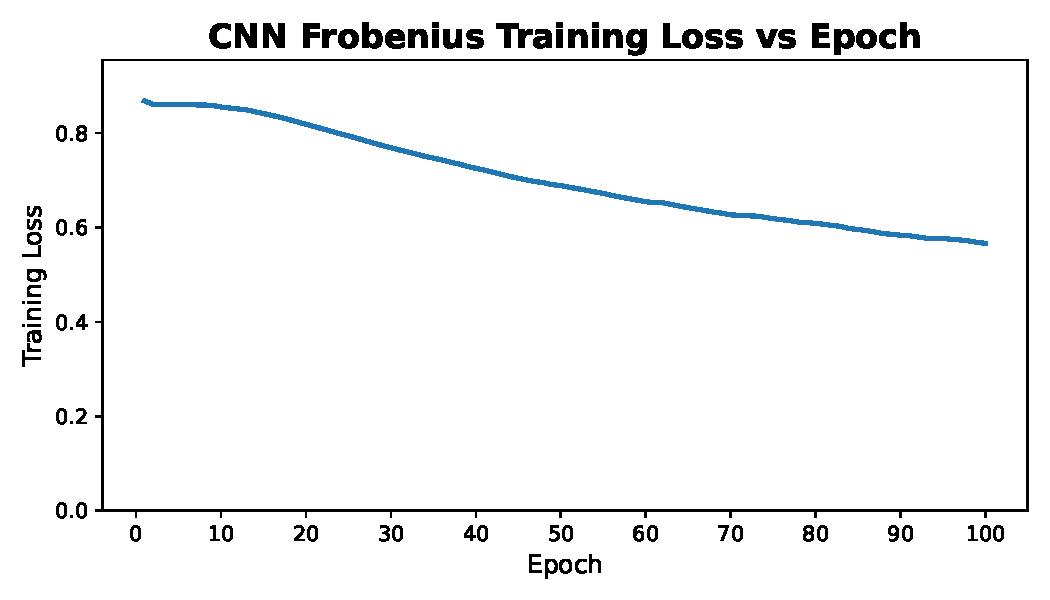
\includegraphics[width=\linewidth]{figures/cnn_frob_train_loss.pdf}
\caption{CNN Frobenius}
\end{subfigure}
\begin{subfigure}{0.45\linewidth}
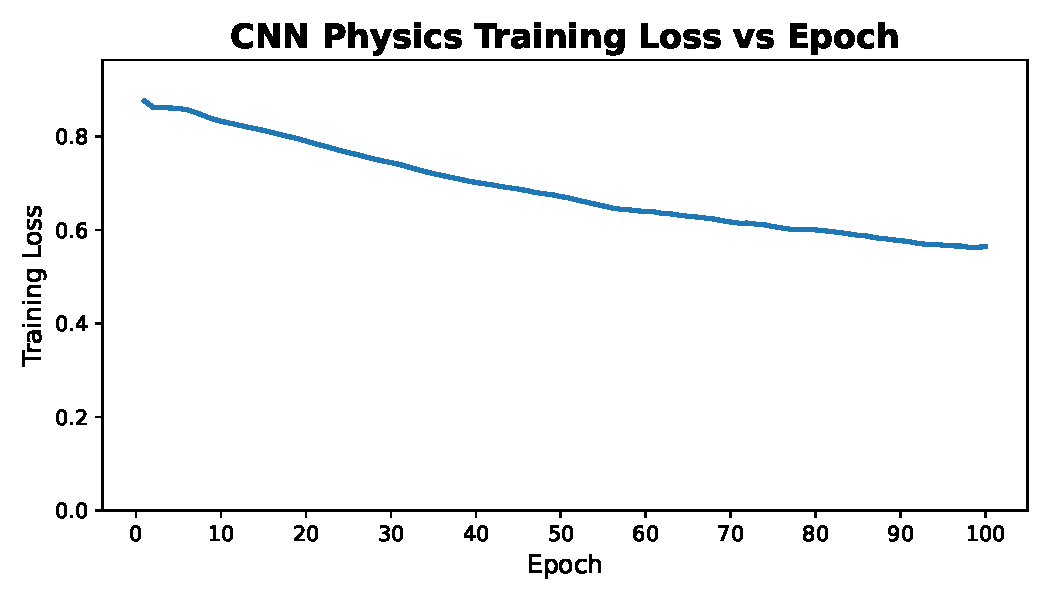
\includegraphics[width=\linewidth]{figures/cnn_physics_train_loss.pdf}
\caption{CNN Physics}
\end{subfigure}

\begin{subfigure}{0.45\linewidth}
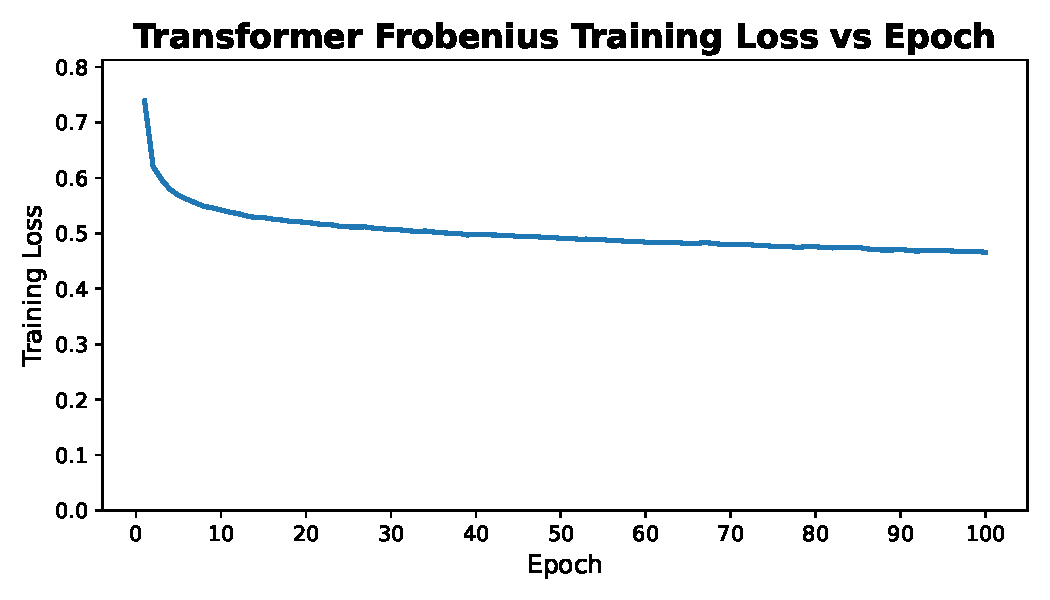
\includegraphics[width=\linewidth]{figures/transformer_frob_train_loss.pdf}
\caption{Transformer Frobenius}
\end{subfigure}
\begin{subfigure}{0.45\linewidth}
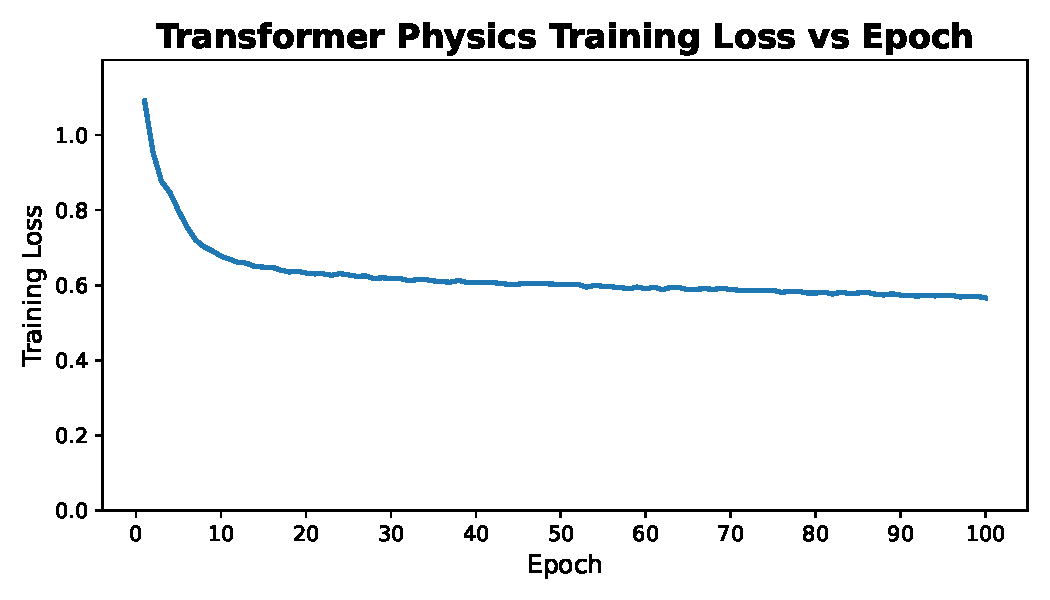
\includegraphics[width=\linewidth]{figures/transformer_physics_train_loss.pdf}
\caption{Transformer Physics}
\end{subfigure}
\end{figure}

\begin{center}
\begin{tabular}{llrrr}
Architecture & Loss Function\footnotemark & Final train loss & Final test loss & Test loss - train loss\\
\hline
CNN & Frobenius & 0.57 & 0.72 & 0.15\\
Transformer & Frobenius & 0.46 & 0.57 & 0.11\\
CNN & Physics & 0.56 & 0.74 & 0.18\\
Transformer & Physics & 0.57 & 0.55 & -0.02\\
\end{tabular}
\end{center}\footnotetext[1]{\label{orge6bd694}Reconstruction losses are only comparable within the same loss family (Frobenius vs. Frobenius, Physics vs. Physics). Cross-family comparisons have no physical meaning.}

Across all four models, we observe clear and stable convergence patterns, but with markedly different learning dynamics between the convolutional and transformer architectures. The CNN-based models exhibit slow, almost linear improvement over the full 100-epoch training horizon. Both CNN variants begin with relatively high reconstruction loss and decrease steadily, with no sharp transitions or instabilities. This behavior is typical of convolutional autoencoders trained on structured but moderately noisy data: the model capacity is modest, gradients are well-behaved, and each pass over the dataset produces small, incremental refinement. Notably, the physics-informed CNN shows a slightly higher and more persistent training loss than its Frobenius counterpart, consistent with the fact that the additional physical penalties restrict the feasible solution space and prevent the network from over-optimizing purely for numerical reconstruction error.

The transformer models behave very differently. Both transformer variants undergo a rapid and steep drop in loss during the first 5–10 epochs, followed by a long plateau phase with only marginal improvements thereafter. This is characteristic of overparameterized attention models: once the model discovers a representation that captures the dominant global correlations, subsequent training mostly fine-tunes local structure and stabilizes the latent space. The physics-informed transformer exhibits a slightly higher early-stage loss due to the additional constraints, but it converges to a value similar to the unconstrained version, suggesting that the transformer’s capacity is large enough to satisfy physical priors without sacrificing reconstruction performance. Importantly, neither transformer shows signs of divergence, mode collapse, or pathological oscillation during training; after the initial sharp transient, the curves flatten and become smooth.

Overall, the training trajectories align well with architectural expectations: CNNs improve slowly but consistently, while transformers learn fast and then saturate. The physics-informed regularization increases training loss for both families, but does not destabilize optimization, and the regularized models converge to values within a small margin of their unconstrained baselines.
\subsubsection{Architecture and Loss Function Comparison}
\label{sec:org9968f0d}
\begin{center}
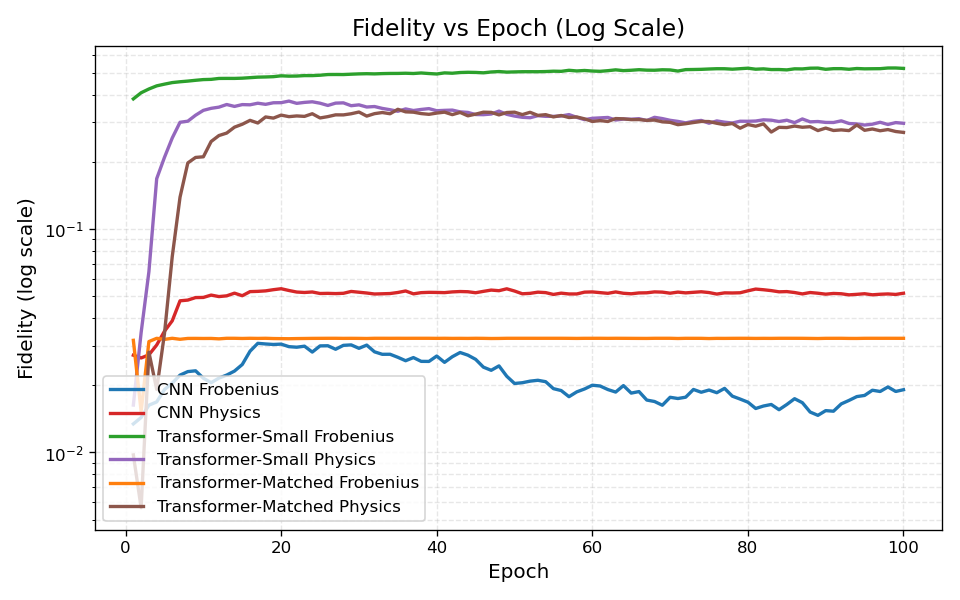
\includegraphics[width=.9\linewidth]{./figures/fidelity_log_combined.png}
\end{center}


\begin{center}
\begin{tabular}{llr}
Architecture & Loss Function & Final fidelity proxy\footnotemark\\
\hline
CNN & Frobenius & 0.02\\
Transformer & Frobenius & 0.52\\
CNN & Physics & 0.05\\
Transformer & Physics & 0.23\\
\end{tabular}
\end{center}\footnotetext[2]{\label{orgf54e31a}The evaluation fidelity is the same normalized Frobenius inner product used as the training loss for Frobenius-trained models. This gives Frobenius-trained models an inherent advantage on this metric, since they directly optimize for it, whereas physics-informed models optimize for a composite objective that includes additional constraints.}

Note that the evaluation fidelity is identical to the training objective for Frobenius-trained models, giving them an inherent advantage over physics-informed models, which optimize a composite loss that includes additional physical constraints.

The fidelity comparison reveals a clear separation in capability between the two architectural families. Models trained with Frobenius loss show the largest gap: the transformer achieves more than an order of magnitude higher fidelity than the CNN. This aligns with the architectural expectation. CNNs operate with strictly local receptive fields, which makes them fundamentally poor at modeling the long-range phase correlations and global coherence patterns that define mixed-state quantum structure. The transformer, which attends across the entire density matrix, has no such bottleneck and therefore captures a much richer portion of the underlying state manifold.

Introducing the physics-informed loss degrades performance for both architectures. On the Frobenius proxy metric, the physics-informed CNN appears to benefit slightly (0.02 to 0.05), but as shown in the Uhlmann fidelity evaluation below, this is misleading: the true quantum fidelity actually decreases. The transformer loses substantial performance when physics constraints are applied. The physics-informed loss penalizes deviations from Hermiticity, unit trace, and PSD, and both architectures respond by collapsing toward generic, low-information "safe" states rather than aggressively reconstructing the underlying quantum structure. The result is physically valid output with significantly reduced alignment to the target state.

Taken together, these results show that (i) transformers are strictly more capable reconstruction models than CNNs for density-matrix denoising, and (ii) physics-informed regularization degrades reconstruction quality for both architectures when measured by true quantum fidelity.
\subsubsection{Uhlmann Fidelity Evaluation}
\label{sec:org2a77a0a}

To verify that these findings are not artifacts of evaluating on the same metric used for training, we additionally evaluated all models on the Uhlmann fidelity, the standard quantum-mechanical measure of state distinguishability. Unlike the normalized Frobenius inner product, the Uhlmann fidelity is not directly optimized by any of the training objectives, providing an unbiased comparison across all four configurations.
\begin{enumerate}
\item Baseline: Noisy Input Fidelity
\label{sec:orgf616f09}

Before evaluating model performance, we establish the baseline fidelity between noisy inputs and clean targets. This quantifies how much information the noise channels destroy and provides context for interpreting model improvements.

\begin{figure}[htbp]
\centering
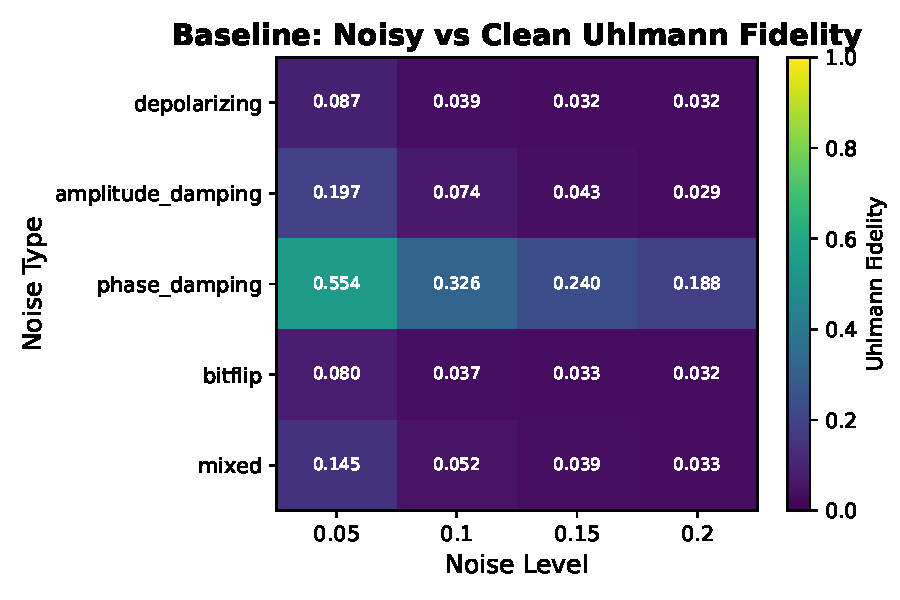
\includegraphics[width=0.6\textwidth]{figures/baseline_noisy_vs_clean_heatmap.pdf}
\caption{\label{fig:orgcaca613}Baseline Uhlmann fidelity between noisy inputs and clean target states across noise types and levels. Lower values indicate more severe corruption.}
\end{figure}

\begin{center}
\begin{tabular}{lrrrr}
Noise Type & p=0.05 & p=0.10 & p=0.15 & p=0.20\\
\hline
Depolarizing & 0.09 & 0.04 & 0.03 & 0.03\\
Amplitude Damping & 0.20 & 0.07 & 0.04 & 0.03\\
Phase Damping & 0.55 & 0.33 & 0.24 & 0.19\\
Bit Flip & 0.08 & 0.04 & 0.03 & 0.03\\
Mixed & 0.14 & 0.05 & 0.04 & 0.03\\
\end{tabular}
\end{center}

The overall baseline fidelity across the test set is \textbf{0.11 ± 0.15}, indicating substantial corruption. Phase damping preserves the most structure (mean 0.33), while depolarizing and bit-flip channels are most destructive (mean 0.05). This establishes that the denoising task is nontrivial: models must recover significant quantum information that has been largely destroyed by the noise process.
\item Model Performance and Improvement
\label{sec:orga29cd05}

\begin{center}
\begin{tabular}{lllr}
Architecture & Loss Function & Uhlmann Fidelity & Improvement over Baseline\\
\hline
Baseline & (Noisy input) & 0.11 ± 0.15 & —\\
CNN & Frobenius & 0.30 ± 0.28 & +0.19\\
Transformer & Frobenius & 0.95 ± 0.12 & +0.84\\
CNN & Physics & 0.06 ± 0.05 & −0.05\\
Transformer & Physics & 0.33 ± 0.33 & +0.22\\
\end{tabular}
\end{center}

\begin{figure}[htbp]
\centering
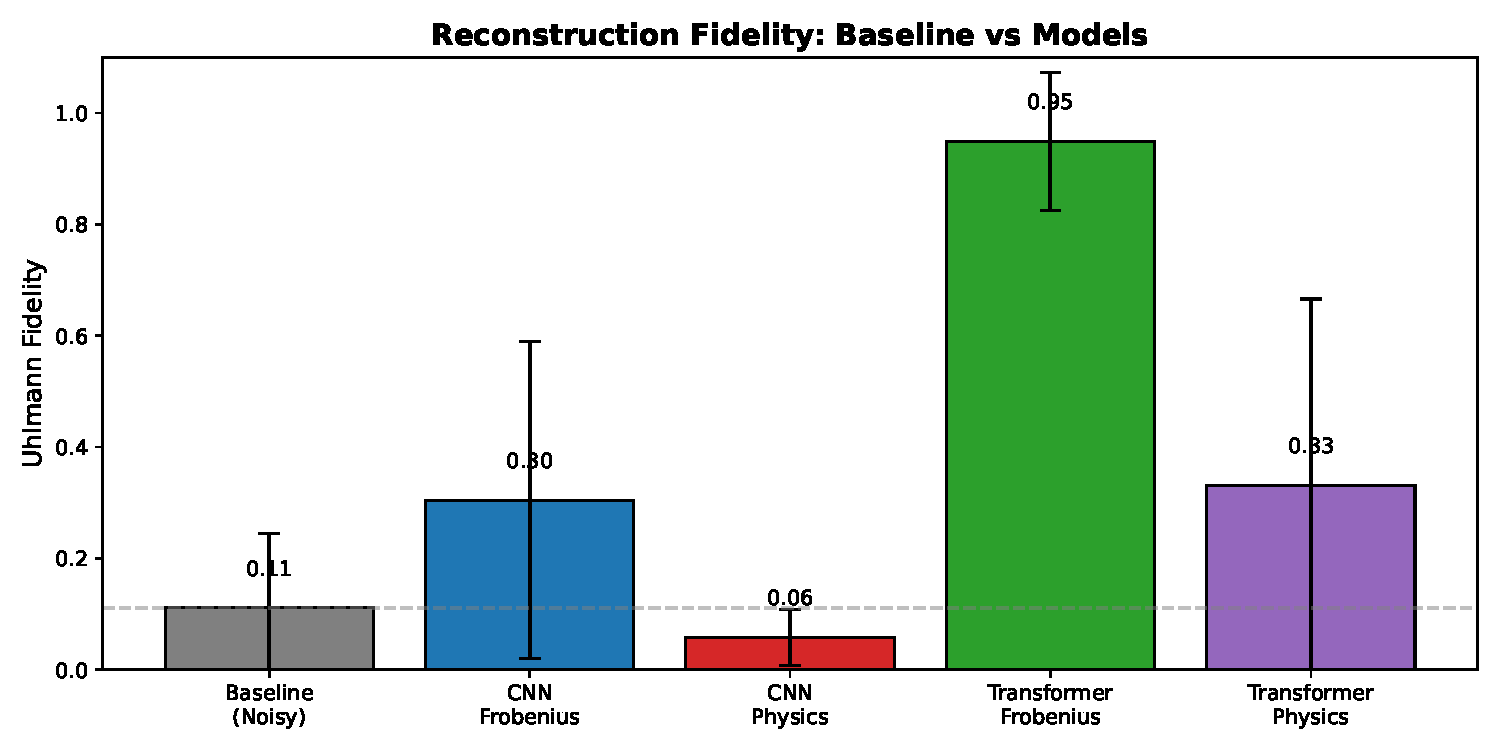
\includegraphics[width=0.8\textwidth]{figures/baseline_vs_models_bar.pdf}
\caption{\label{fig:orgeff333c}Reconstruction fidelity comparison. The baseline (gray) shows the fidelity of noisy inputs to clean targets. The Frobenius-trained transformer achieves near-perfect reconstruction (+0.84 improvement), while the physics-informed CNN performs worse than doing nothing.}
\end{figure}

The Frobenius-trained transformer achieves 0.95 mean fidelity, an improvement of +0.84 over the noisy baseline—recovering nearly all of the quantum information destroyed by the noise channels. The Frobenius-trained CNN provides a modest +0.19 improvement, while the physics-informed transformer achieves +0.22. Most strikingly, the physics-informed CNN achieves only 0.06 fidelity, which is \textbf{worse than the noisy input itself} (−0.05). This indicates that the physics constraints, rather than guiding the model toward valid reconstructions, cause it to collapse toward generic low-fidelity states that happen to satisfy Hermiticity, trace, and positivity constraints.
\item Improvement by Noise Type
\label{sec:orgf1a650e}

\begin{figure}[h!]
\centering
\begin{subfigure}{0.45\linewidth}
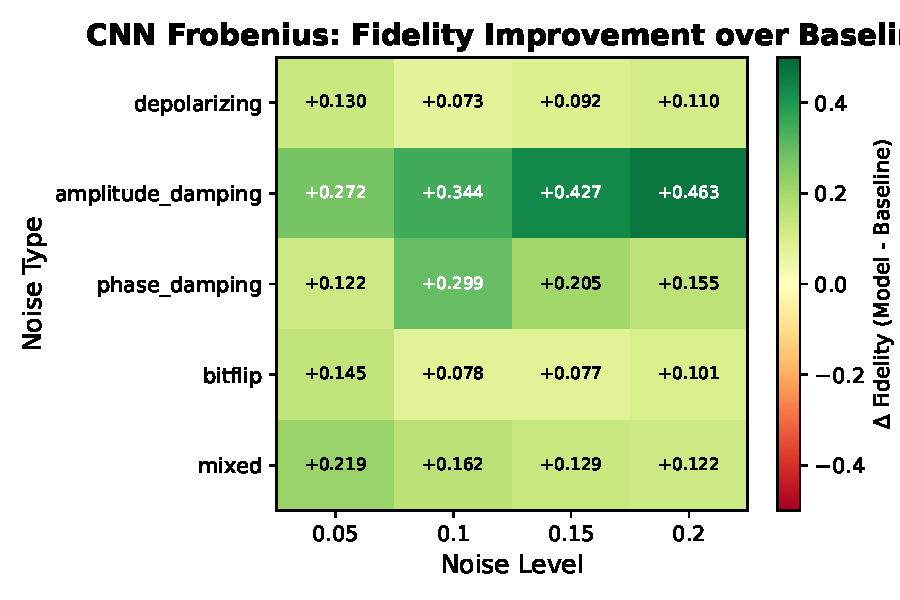
\includegraphics[width=\linewidth]{figures/cnn_frob_improvement_heatmap.pdf}
\caption{CNN Frobenius}
\end{subfigure}
\begin{subfigure}{0.45\linewidth}
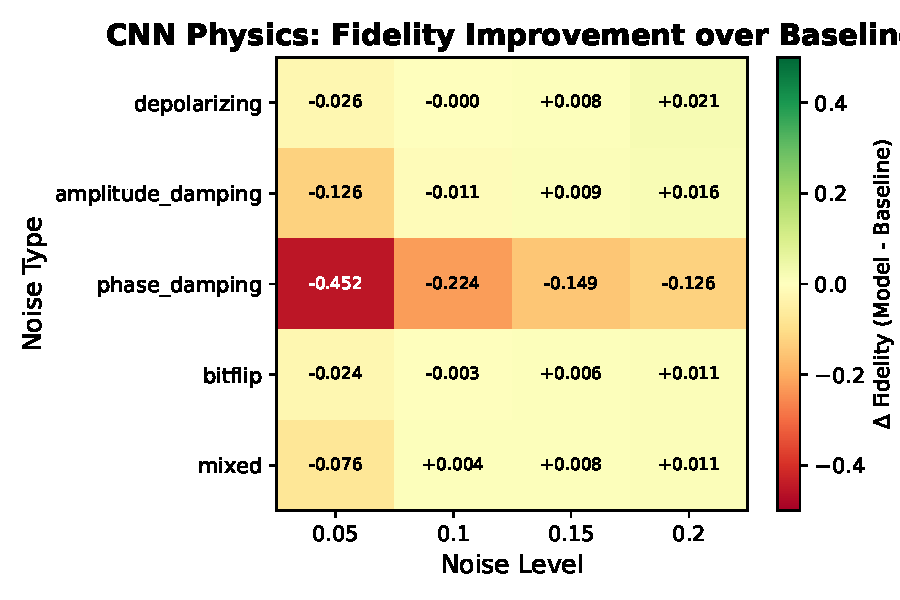
\includegraphics[width=\linewidth]{figures/cnn_physics_improvement_heatmap.pdf}
\caption{CNN Physics}
\end{subfigure}

\begin{subfigure}{0.45\linewidth}
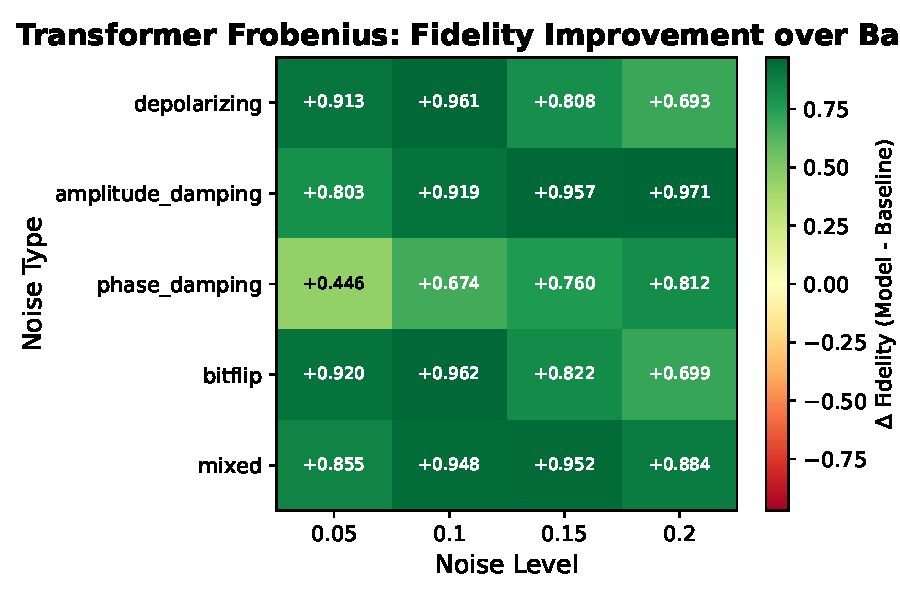
\includegraphics[width=\linewidth]{figures/transformer_frob_improvement_heatmap.pdf}
\caption{Transformer Frobenius}
\end{subfigure}
\begin{subfigure}{0.45\linewidth}
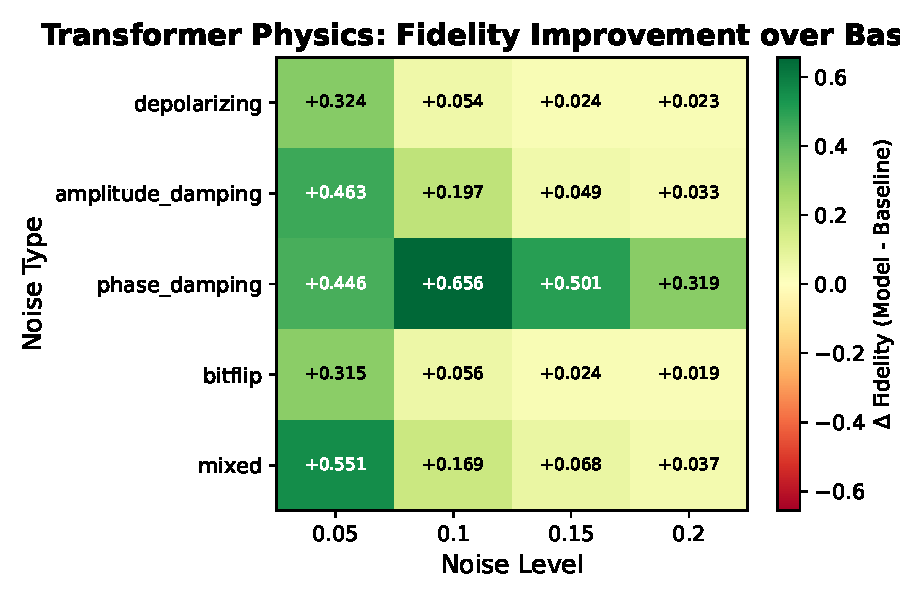
\includegraphics[width=\linewidth]{figures/transformer_physics_improvement_heatmap.pdf}
\caption{Transformer Physics}
\end{subfigure}
\caption{Fidelity improvement over baseline (model fidelity minus noisy input fidelity) by noise type and level. Green indicates improvement; red indicates degradation. The Frobenius-trained transformer shows consistent large improvements across all conditions, while the physics-informed CNN shows degradation (red) in most cells.}
\label{fig:improvement-heatmaps}
\end{figure}

The improvement heatmaps reveal that the Frobenius-trained transformer consistently improves fidelity across all noise types and levels, with gains exceeding +0.5 in most cells. The physics-informed CNN shows widespread degradation (negative improvement), confirming that its outputs are systematically worse than simply using the noisy input. This finding has practical implications: physics-informed regularization should not be applied blindly, as it can cause models to produce outputs that are physically valid but informationally useless.

These results validate the architectural conclusions on a neutral metric: transformers dramatically outperform CNNs regardless of evaluation measure, and physics-informed regularization degrades reconstruction quality for both architectures when measured by true quantum fidelity.
\newpage
\end{enumerate}
\subsubsection{Noise-type and Noise-Level Comparison}
\label{sec:org9579a07}
\begin{figure}[h!]
\centering
\begin{subfigure}{0.45\linewidth}
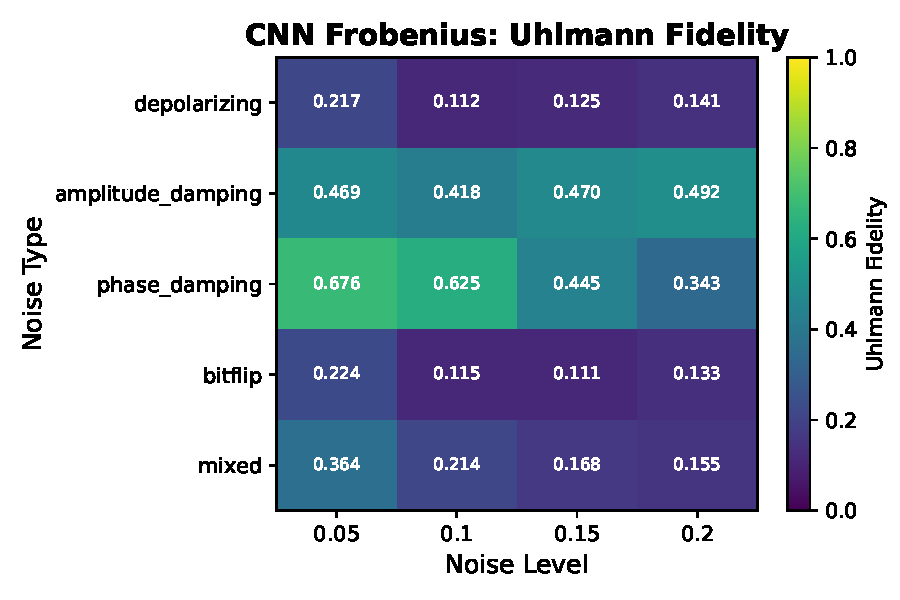
\includegraphics[width=\linewidth]{figures/cnn_frob_noise_cells_heatmap.pdf}
\caption{CNN Frobenius}
\end{subfigure}
\begin{subfigure}{0.45\linewidth}
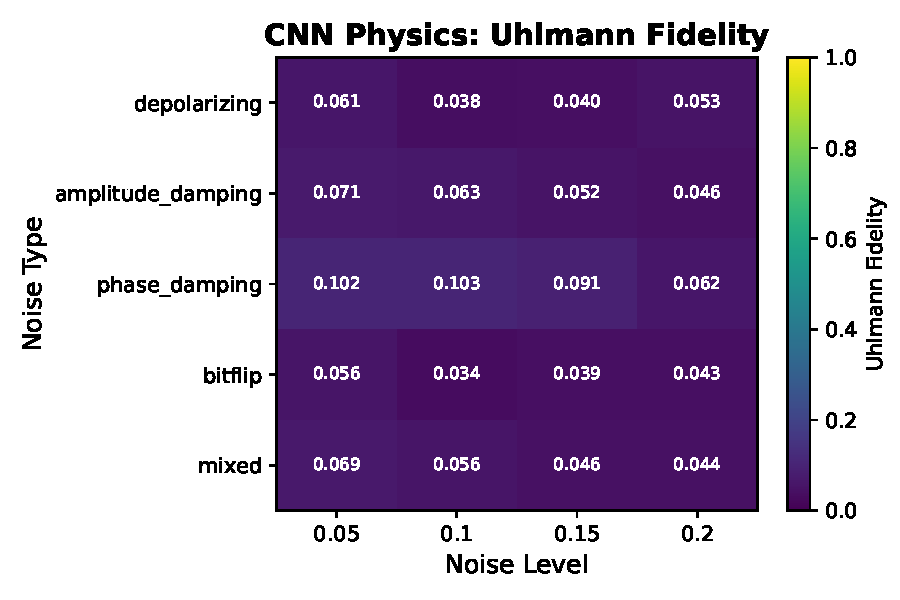
\includegraphics[width=\linewidth]{figures/cnn_physics_noise_cells_heatmap.pdf}
\caption{CNN Physics}
\end{subfigure}

\begin{subfigure}{0.45\linewidth}
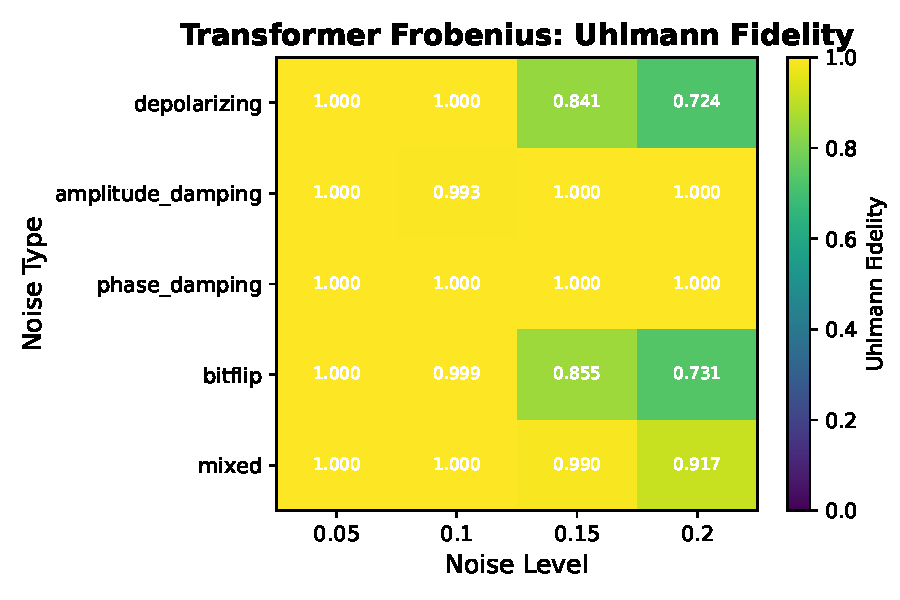
\includegraphics[width=\linewidth]{figures/transformer_frob_noise_cells_heatmap.pdf}
\caption{Transformer Frobenius}
\end{subfigure}
\begin{subfigure}{0.45\linewidth}
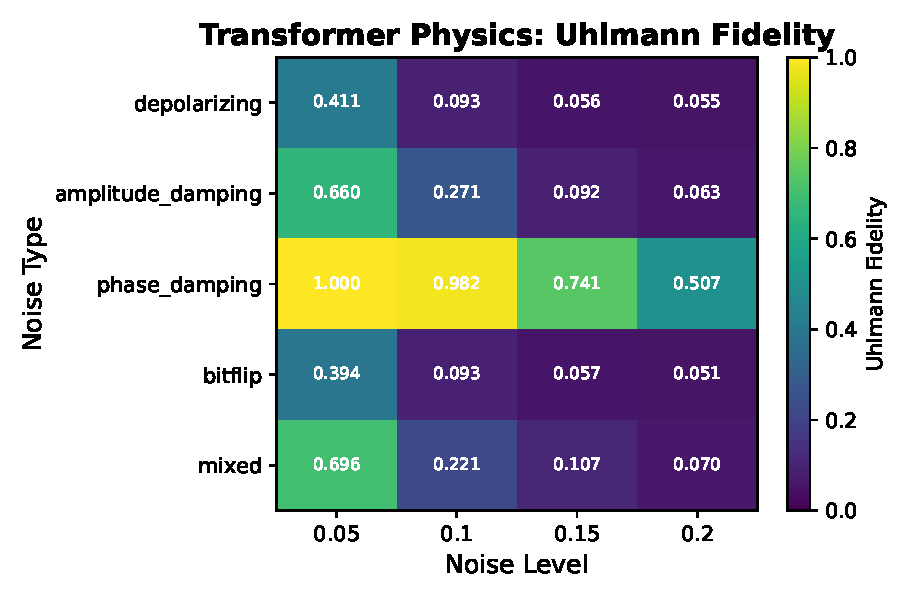
\includegraphics[width=\linewidth]{figures/transformer_physics_noise_cells_heatmap.pdf}
\caption{Transformer Physics}
\end{subfigure}
\end{figure}
Across all architectures, fidelity varies systematically with both noise type and noise level, revealing clear differences in robustness among the four models. The CNN models achieve only marginal fidelity overall and show weak sensitivity to noise type, with values typically in the 0.02 to 0.05 range regardless of corruption. In contrast, the Transformer architectures display structured behavior: the Frobenius-loss Transformer consistently achieves the highest fidelity across nearly every noise cell, particularly for low-level phase damping and mixed noise, where it reaches its best performance. Its fidelity decays as the noise level increases, but it remains substantially above all CNN baselines. The physics-informed Transformer shows the opposite pattern. Although its absolute fidelity is lower than the Frobenius variant, it is markedly more stable across noise types and noise levels, exhibiting much smaller drops in fidelity as corruption increases. Notably, the physics-informed Transformer performs best on phase damping at low noise levels (0.05 and 0.10); this is likely because phase damping selectively destroys off-diagonal coherences while preserving diagonal populations, trace, and Hermiticity, meaning the corrupted state already satisfies the physics constraints and the regularization does not interfere with reconstruction. This indicates that the constraints enforced by the physics-informed loss improve robustness in high-noise regimes at the cost of peak performance in cleaner settings. Overall, these noise-resolved results show that Transformers not only outperform CNNs in denoising fidelity but also capture structure in the noise process itself, with the Frobenius variant excelling in low-noise cells and the physics-informed variant maintaining comparatively consistent behavior under stronger corruptions.
\subsubsection{Failure Modes and Qualitative Analysis}
\label{sec:orgb603441}
A closer inspection of individual reconstruction failures reveals distinct failure modes tied to both architecture and loss design. The CNN models exhibit the most brittle behavior: when they fail, they typically collapse toward oversmoothed density matrices with attenuated off-diagonal structure, especially under high noise levels. This is consistent with their convolutional inductive bias, which cannot easily represent long-range correlations in the density matrix. The Frobenius-loss CNN is especially prone to this collapse, while the physics-informed CNN occasionally produces outputs that satisfy physical constraints but remain far from the true clean states, indicating that the added constraints can steer optimization without meaningfully improving reconstruction. The Transformer models fail in more structured ways. The Frobenius-loss Transformer sometimes produces sharp but globally misaligned reconstructions, suggesting that it has learned expressive global patterns but can be destabilized under heavy noise. The physics-informed Transformer exhibits the most “graceful” failures: even when fidelity drops, its outputs tend to retain Hermiticity, a well-formed eigenvalue spectrum, and approximately correct trace, confirming that the loss constraints operate as intended. These qualitative differences underline that architectural capacity governs how a model fails, while the loss function governs how bad those failures become.
\section{Conclusion}
\label{sec:orgc7e311f}
This work compared four machine learning strategies for density-matrix denoising and demonstrated that architectural choice is the dominant factor in reconstruction quality. The Frobenius-trained transformer achieved 0.95 Uhlmann fidelity on the test set, approaching near-perfect state reconstruction, while all other configurations remained below 0.35. This result was validated on the Uhlmann fidelity, a standard quantum-mechanical measure that none of the training objectives directly optimize, confirming that the transformer's superiority is not an artifact of metric alignment.

Contrary to initial expectations, physics-informed regularization degraded performance for both architectures when evaluated on true quantum fidelity. The physics-informed CNN achieved only 0.06 Uhlmann fidelity compared to 0.30 for its Frobenius-trained counterpart, and the physics-informed transformer dropped from 0.95 to 0.33. While the physics constraints successfully enforce structural validity (Hermiticity, unit trace, positive semidefiniteness), they do so at the expense of accurate state reconstruction. The regularization appears to push models toward generic, low-information outputs that satisfy physical axioms but fail to capture the specific structure of the target state.

These findings have practical implications for quantum error mitigation. First, transformer architectures with global attention are fundamentally better suited to density-matrix denoising than CNNs, whose local receptive fields cannot capture the nonlocal correlations inherent to quantum states. Second, soft physics constraints applied during training are counterproductive when the goal is high-fidelity reconstruction; if physical validity is required, post-hoc projection onto the valid state manifold may be preferable to regularization. Third, evaluation on training-aligned metrics can be misleading, and neutral measures like Uhlmann fidelity should be reported alongside proxy losses.

Improving classical denoisers directly increases the effective reliability of near-term quantum experiments. The transformer architecture identified here offers a practical path toward extracting higher-quality results from noisy intermediate-scale quantum hardware, reducing the measurement overhead required for useful computation while fault-tolerant systems remain out of reach.
\section{References}
\label{sec:org79acb40}
\printbibliography
\subsection{{\bfseries\sffamily TODO} Add more citations}
\label{sec:org50230ca}
\section{Appendix}
\label{sec:org157bf4c}
\end{document}
